% ==========================================================================================
% ==========================================================================================
% ==========================================================================================
\RequirePackage[l2tabu, orthodox]{nag}

\def\myname{John Terhorst}
\def\myshortname{Terhorst, J.}
\def\mydoctitle{Document Title}
\def\myfontsize{10pt}
\def\mymargins{1.6in}

% ==========================================================================================
% ==========================================================================================
% ==========================================================================================

\documentclass[letterpaper,\myfontsize]{article}
%\documentclass[letterpaper,titlepage,\myfontsize]{article}
%\documentclass[letterpaper,twocolumn,\myfontsize]{article}
%\usepackage[top=\mymargins, bottom=\mymargins, left=\mymargins, right=\mymargins]{geometry} % showframe
%\usepackage{typearea} % auto-calculate page layout
% \renewcommand{\familydefault}{\sfdefault} % sans default 
% \DeclareFontSeriesDefault[rm]{bf}{b} % when in roman family, define bfseries as b {not bx}
% \frenchspacing %disables extra spacing after periods

% ==========================================================================================
% ==========================================================================================
% ==========================================================================================

% basic setup - for font packages see http://www.tug.dk/FontCatalogue/

% \renewcommand{\familydefault}{\sfdefault}   % \rmdefault, \sfdefault, \ttdefault
% \usepackage[T1]{fontenc} % use for documents with lots of accented chars like \"o or \AA or \'e
% \usepackage[tracking=true,kerning=true,factor=1100,stretch=10,shrink=10]{microtype}
\usepackage{microtype,verbatim} % mlmodern
\usepackage{mlmodern}
\usepackage{graphicx}
%\usepackage{txfonts} % use times with math support
%\usepackage{mathptmx} % use times with math support  
%\usepackage{newtxtext,newtxmath} % use times with math support 
% \usepackage[smallerops,subscriptcorrection]{newtxmath} 
% \usepackage[minionint,lf]{MinionPro} % use minionpro with math support
%\usepackage{anyfontsize}
%\usepackage{authoraftertitle} % access \MyTitle etc
\usepackage[version=4]{mhchem}  % use arrows=pgf-filled if using mathptmx or newtxtext/newtxmath
%\usepackage{parskip}
\usepackage{siunitx}
\usepackage{textgreek} % upright greek in text mode; eg \textalpha. use [artemisia] for tmx or [euler] for pazo
% \usepackage{mathtools} % replaces amsmath/symb
% \usepackage{ulem} % use underline for \emph{}; provides better \uline{}; use [normalem] to keep \emph{} as italic
% textcomp,float % other utility packages
% \usepackage[shortlabels]{enumitem} % can use [noitemsep] in itemize
% \usepackage{paralist} inparaenum 
% \usepackage[all]{nowidow} % widow/orphan prevention
% \usepackage[bottom,hang]{footmisc}\setlength\footnotemargin{9pt}\interfootnotelinepenalty=10000\setlength{\skip\footins}{0.5cm}
% \usepackage{setspace} % provides \doublespacing, \onehalfspacing, and \setstetch{}
% or just use eg \linespread{1.1}
% ==========================================================================================
% ==========================================================================================
% ==========================================================================================

% references

\begin{comment}
% natbib 
\usepackage[super,comma,sort&compress]{natbib}
\renewcommand{\bibnumfmt}[1]{#1.}
% \renewcommand{\refname}{References}
% \renewcommand{\bibname}{References}
% use with:
% \addcontentsline{toc}{chapter}{References}
% \bibliographystyle{jpt-all} % see other bst files in bibtex folder % or don't declare if using achemso
% \bibliography{refsdiss} % bibfile
% or for manual referencing:   key      journal      year        vol       page
\newcommand*\myaref[6]{\bibitem{#1}#2 \textit{#3} \textbf{#4}, \textit{#5}, #6.} 
\newcommand*\mytref[7]{\bibitem{#1}#2 ``#3.'' \textit{#4} \textbf{#5}, \textit{#6}, #7.} % with title
\newcommand*\myzref[8]{\bibitem{#1}#2 ``#3.'' \textit{#4} \textbf{#5}, \textit{#6}(#7), #8.} % with title and issue
\end{comment}

 % biber/biblatex - using custom.bbx/cbx files from acs

\usepackage[autocite = superscript, sortcites = true, backend = biber, style = custom]{biblatex}\bibliography{bibrefs}
    \defbibenvironment{bibliography}
      {\enumerate
          {}
          {\setlength{\leftmargin}{\bibhang}%
          \setlength{\itemindent}{-\leftmargin}%
          \setlength{\itemsep}{\bibitemsep}%
          \setlength{\parsep}{\bibparsep}}}
      {\endenumerate}
      {\item}
    \DeclareCiteCommand{\citenum}
      {}
      {\printfield{labelnumber}}
      {}
      {}

% roman footnotes so we don't conflict with bib references
\renewcommand{\thefootnote}{\textit{\roman{footnote}}}
\usepackage[bottom]{footmisc}\interfootnotelinepenalty=10000\setlength{\skip\footins}{0.5cm} 
%\end{comment}

% use with
\begin{comment}
\begin{refsection}
\printbibliography[heading=subbibliography]
\end{refsection}
\end{comment}
% or just \printbibliography

% sections and toc depth
\setcounter{secnumdepth}{4}%\setcounter{tocdepth}{4}

% ==========================================================================================
% ==========================================================================================
% ==========================================================================================

% tables and figures

\usepackage{booktabs}
\setlength\heavyrulewidth{0.15ex}\setlength\cmidrulewidth{0.1ex}\setlength\lightrulewidth{0.1ex}

%\usepackage[font=normalsize,labelfont={bf},margin=1in]{caption}\captionsetup[table]{aboveskip=3pt}\captionsetup[figure]{skip=3pt}
\usepackage[font=normalsize,labelfont={sc}]{caption}\captionsetup[table]{aboveskip=3pt}\captionsetup[figure]{skip=3pt}
% \setlength{\textfloatsep}{9pt plus 1.0pt minus 2.0pt} % adjust space from caption to body text

% standard figure env - floating. can use \usepackage{float} with [H] to not float
\begin{comment}
\begin{figure}[htbp]
	\centering
		\includegraphics[width=\textwidth]{bornrad.pdf} % scale % or do \input{} for tex/tikz
		\caption{The pairwise nature of the Born radius.}
		\label{fig:bornrad}
\end{figure}
\end{comment}

% to do a figure without the env, use this with \usepackage{caption} 

\begin{comment}
\begin{center}
\resizebox{\textwidth}{!}{% code generated by https://www.mathcha.io/editor#


% Gradient Info
  
\tikzset {_fl3j1z7ci/.code = {\pgfsetadditionalshadetransform{ \pgftransformshift{\pgfpoint{0 bp } { 0 bp }  }  \pgftransformscale{1 }  }}}
\pgfdeclareradialshading{_ajvec99hy}{\pgfpoint{0bp}{0bp}}{rgb(0bp)=(0,0,0);
rgb(0.17857142857142858bp)=(0,0,0);
rgb(25bp)=(1,1,1);
rgb(400bp)=(1,1,1)}
\tikzset{_c47t8m2b3/.code = {\pgfsetadditionalshadetransform{\pgftransformshift{\pgfpoint{0 bp } { 0 bp }  }  \pgftransformscale{1 } }}}
\pgfdeclareradialshading{_kz6fsyt8x} { \pgfpoint{0bp} {0bp}} {color(0bp)=(transparent!27);
color(0.17857142857142858bp)=(transparent!27);
color(25bp)=(transparent!0);
color(400bp)=(transparent!0)} 
\pgfdeclarefading{_sdra5fwgv}{\tikz \fill[shading=_kz6fsyt8x,_c47t8m2b3] (0,0) rectangle (50bp,50bp); } 
\tikzset{every picture/.style={line width=0.65pt}} %set default line width to 0.75pt        

\begin{tikzpicture}[x=0.75pt,y=0.75pt,yscale=-1,xscale=1]
%uncomment if require: \path (0,300); %set diagram left start at 0, and has height of 300

%Shape: Circle [id:dp5031363586176847] 
\draw  [fill={rgb, 255:red, 0; green, 0; blue, 0 }  ,fill opacity=1 ] (353.67,159.68) .. controls (353.67,157.75) and (355.23,156.18) .. (357.17,156.18) .. controls (359.1,156.18) and (360.67,157.75) .. (360.67,159.68) .. controls (360.67,161.61) and (359.1,163.18) .. (357.17,163.18) .. controls (355.23,163.18) and (353.67,161.61) .. (353.67,159.68) -- cycle ;
%Shape: Circle [id:dp6021592429793765] 
\draw  [fill={rgb, 255:red, 225; green, 225; blue, 225 }  ,fill opacity=1 ] (345,159.33) .. controls (345,157.4) and (346.57,155.83) .. (348.5,155.83) .. controls (350.43,155.83) and (352,157.4) .. (352,159.33) .. controls (352,161.27) and (350.43,162.83) .. (348.5,162.83) .. controls (346.57,162.83) and (345,161.27) .. (345,159.33) -- cycle ;
%Shape: Circle [id:dp03262422408388033] 
\path  [shading=_ajvec99hy,_fl3j1z7ci,path fading= _sdra5fwgv ,fading transform={xshift=2}] (200,203.5) .. controls (200,176.53) and (221.86,154.67) .. (248.83,154.67) .. controls (275.8,154.67) and (297.67,176.53) .. (297.67,203.5) .. controls (297.67,230.47) and (275.8,252.33) .. (248.83,252.33) .. controls (221.86,252.33) and (200,230.47) .. (200,203.5) -- cycle ; % for fading 
 \draw  [color={rgb, 255:red, 255; green, 255; blue, 255 }  ,draw opacity=1 ] (200,203.5) .. controls (200,176.53) and (221.86,154.67) .. (248.83,154.67) .. controls (275.8,154.67) and (297.67,176.53) .. (297.67,203.5) .. controls (297.67,230.47) and (275.8,252.33) .. (248.83,252.33) .. controls (221.86,252.33) and (200,230.47) .. (200,203.5) -- cycle ; % for border 

%Shape: Circle [id:dp6125886336785793] 
\draw  [fill={rgb, 255:red, 0; green, 0; blue, 0 }  ,fill opacity=1 ] (247.37,202.04) .. controls (247.37,201.23) and (248.02,200.57) .. (248.83,200.57) .. controls (249.64,200.57) and (250.3,201.23) .. (250.3,202.04) .. controls (250.3,202.84) and (249.64,203.5) .. (248.83,203.5) .. controls (248.02,203.5) and (247.37,202.84) .. (247.37,202.04) -- cycle ;
%Shape: Rectangle [id:dp737374784788116] 
\draw   (320,150) -- (390,150) -- (390,182.36) -- (320,182.36) -- cycle ;
%Straight Lines [id:da9404773687410686] 
\draw [fill={rgb, 255:red, 255; green, 255; blue, 255 }  ,fill opacity=1 ]   (320,150) -- (320,182.36) -- (248.83,202.04) ;
%Shape: Polygon [id:ds005534302931645474] 
\draw  [fill={rgb, 255:red, 255; green, 255; blue, 255 }  ,fill opacity=1 ] (320,182.36) -- (390,182.36) -- (248.83,202.04) -- cycle ;
%Shape: Circle [id:dp39755043985132055] 
\draw  [fill={rgb, 255:red, 0; green, 0; blue, 0 }  ,fill opacity=1 ] (344,163.83) .. controls (344,161.9) and (345.57,160.33) .. (347.5,160.33) .. controls (349.43,160.33) and (351,161.9) .. (351,163.83) .. controls (351,165.77) and (349.43,167.33) .. (347.5,167.33) .. controls (345.57,167.33) and (344,165.77) .. (344,163.83) -- cycle ;
%Shape: Circle [id:dp4473204849748251] 
\draw  [fill={rgb, 255:red, 225; green, 225; blue, 225 }  ,fill opacity=1 ] (348,166.51) .. controls (348,164.58) and (349.57,163.01) .. (351.5,163.01) .. controls (353.43,163.01) and (355,164.58) .. (355,166.51) .. controls (355,168.45) and (353.43,170.01) .. (351.5,170.01) .. controls (349.57,170.01) and (348,168.45) .. (348,166.51) -- cycle ;
%Shape: Circle [id:dp4488461328919484] 
\draw  [fill={rgb, 255:red, 0; green, 0; blue, 0 }  ,fill opacity=1 ] (349,161.5) .. controls (349,159.57) and (350.57,158) .. (352.5,158) .. controls (354.43,158) and (356,159.57) .. (356,161.5) .. controls (356,163.43) and (354.43,165) .. (352.5,165) .. controls (350.57,165) and (349,163.43) .. (349,161.5) -- cycle ;
%Shape: Circle [id:dp7389549254976258] 
\draw  [fill={rgb, 255:red, 225; green, 225; blue, 225 }  ,fill opacity=1 ] (353.67,163.18) .. controls (353.67,161.25) and (355.23,159.68) .. (357.17,159.68) .. controls (359.1,159.68) and (360.67,161.25) .. (360.67,163.18) .. controls (360.67,165.11) and (359.1,166.68) .. (357.17,166.68) .. controls (355.23,166.68) and (353.67,165.11) .. (353.67,163.18) -- cycle ;
%Shape: Circle [id:dp479134066231107] 
\draw  [fill={rgb, 255:red, 0; green, 0; blue, 0 }  ,fill opacity=1 ] (344.5,170.01) .. controls (344.5,168.08) and (346.07,166.51) .. (348,166.51) .. controls (349.93,166.51) and (351.5,168.08) .. (351.5,170.01) .. controls (351.5,171.95) and (349.93,173.51) .. (348,173.51) .. controls (346.07,173.51) and (344.5,171.95) .. (344.5,170.01) -- cycle ;
%Shape: Circle [id:dp4479985418514103] 
\draw  [fill={rgb, 255:red, 225; green, 225; blue, 225 }  ,fill opacity=1 ] (340.5,167.33) .. controls (340.5,165.4) and (342.07,163.83) .. (344,163.83) .. controls (345.93,163.83) and (347.5,165.4) .. (347.5,167.33) .. controls (347.5,169.27) and (345.93,170.83) .. (344,170.83) .. controls (342.07,170.83) and (340.5,169.27) .. (340.5,167.33) -- cycle ;
%Shape: Circle [id:dp7971297276833167] 
\draw  [fill={rgb, 255:red, 0; green, 0; blue, 0 }  ,fill opacity=1 ] (353.67,166.68) .. controls (353.67,164.75) and (355.23,163.18) .. (357.17,163.18) .. controls (359.1,163.18) and (360.67,164.75) .. (360.67,166.68) .. controls (360.67,168.61) and (359.1,170.18) .. (357.17,170.18) .. controls (355.23,170.18) and (353.67,168.61) .. (353.67,166.68) -- cycle ;
%Shape: Circle [id:dp5729729111609032] 
\draw  [fill={rgb, 255:red, 225; green, 225; blue, 225 }  ,fill opacity=1 ] (349.5,172) .. controls (349.5,170.07) and (351.07,168.5) .. (353,168.5) .. controls (354.93,168.5) and (356.5,170.07) .. (356.5,172) .. controls (356.5,173.93) and (354.93,175.5) .. (353,175.5) .. controls (351.07,175.5) and (349.5,173.93) .. (349.5,172) -- cycle ;
%Shape: Circle [id:dp07629231382977153] 
\draw  [fill={rgb, 255:red, 0; green, 0; blue, 0 }  ,fill opacity=1 ] (353,172) .. controls (353,170.07) and (354.57,168.5) .. (356.5,168.5) .. controls (358.43,168.5) and (360,170.07) .. (360,172) .. controls (360,173.93) and (358.43,175.5) .. (356.5,175.5) .. controls (354.57,175.5) and (353,173.93) .. (353,172) -- cycle ;
%Shape: Circle [id:dp14599951094051478] 
\draw  [fill={rgb, 255:red, 225; green, 225; blue, 225 }  ,fill opacity=1 ] (357.17,170.18) .. controls (357.17,168.25) and (358.73,166.68) .. (360.67,166.68) .. controls (362.6,166.68) and (364.17,168.25) .. (364.17,170.18) .. controls (364.17,172.11) and (362.6,173.68) .. (360.67,173.68) .. controls (358.73,173.68) and (357.17,172.11) .. (357.17,170.18) -- cycle ;
%Straight Lines [id:da98323072818843] 
\draw    (248.83,202.04) -- (320,150) ;




\end{tikzpicture}
} % to scale \input{} figure based on geometry
\captionof{figure}{Ions.}
\label{fig:ion}
\end{center}

\begin{center}
\scalebox{.75}{% code generated by https://www.mathcha.io/editor#


% Gradient Info
  
\tikzset {_fl3j1z7ci/.code = {\pgfsetadditionalshadetransform{ \pgftransformshift{\pgfpoint{0 bp } { 0 bp }  }  \pgftransformscale{1 }  }}}
\pgfdeclareradialshading{_ajvec99hy}{\pgfpoint{0bp}{0bp}}{rgb(0bp)=(0,0,0);
rgb(0.17857142857142858bp)=(0,0,0);
rgb(25bp)=(1,1,1);
rgb(400bp)=(1,1,1)}
\tikzset{_c47t8m2b3/.code = {\pgfsetadditionalshadetransform{\pgftransformshift{\pgfpoint{0 bp } { 0 bp }  }  \pgftransformscale{1 } }}}
\pgfdeclareradialshading{_kz6fsyt8x} { \pgfpoint{0bp} {0bp}} {color(0bp)=(transparent!27);
color(0.17857142857142858bp)=(transparent!27);
color(25bp)=(transparent!0);
color(400bp)=(transparent!0)} 
\pgfdeclarefading{_sdra5fwgv}{\tikz \fill[shading=_kz6fsyt8x,_c47t8m2b3] (0,0) rectangle (50bp,50bp); } 
\tikzset{every picture/.style={line width=0.65pt}} %set default line width to 0.75pt        

\begin{tikzpicture}[x=0.75pt,y=0.75pt,yscale=-1,xscale=1]
%uncomment if require: \path (0,300); %set diagram left start at 0, and has height of 300

%Shape: Circle [id:dp5031363586176847] 
\draw  [fill={rgb, 255:red, 0; green, 0; blue, 0 }  ,fill opacity=1 ] (353.67,159.68) .. controls (353.67,157.75) and (355.23,156.18) .. (357.17,156.18) .. controls (359.1,156.18) and (360.67,157.75) .. (360.67,159.68) .. controls (360.67,161.61) and (359.1,163.18) .. (357.17,163.18) .. controls (355.23,163.18) and (353.67,161.61) .. (353.67,159.68) -- cycle ;
%Shape: Circle [id:dp6021592429793765] 
\draw  [fill={rgb, 255:red, 225; green, 225; blue, 225 }  ,fill opacity=1 ] (345,159.33) .. controls (345,157.4) and (346.57,155.83) .. (348.5,155.83) .. controls (350.43,155.83) and (352,157.4) .. (352,159.33) .. controls (352,161.27) and (350.43,162.83) .. (348.5,162.83) .. controls (346.57,162.83) and (345,161.27) .. (345,159.33) -- cycle ;
%Shape: Circle [id:dp03262422408388033] 
\path  [shading=_ajvec99hy,_fl3j1z7ci,path fading= _sdra5fwgv ,fading transform={xshift=2}] (200,203.5) .. controls (200,176.53) and (221.86,154.67) .. (248.83,154.67) .. controls (275.8,154.67) and (297.67,176.53) .. (297.67,203.5) .. controls (297.67,230.47) and (275.8,252.33) .. (248.83,252.33) .. controls (221.86,252.33) and (200,230.47) .. (200,203.5) -- cycle ; % for fading 
 \draw  [color={rgb, 255:red, 255; green, 255; blue, 255 }  ,draw opacity=1 ] (200,203.5) .. controls (200,176.53) and (221.86,154.67) .. (248.83,154.67) .. controls (275.8,154.67) and (297.67,176.53) .. (297.67,203.5) .. controls (297.67,230.47) and (275.8,252.33) .. (248.83,252.33) .. controls (221.86,252.33) and (200,230.47) .. (200,203.5) -- cycle ; % for border 

%Shape: Circle [id:dp6125886336785793] 
\draw  [fill={rgb, 255:red, 0; green, 0; blue, 0 }  ,fill opacity=1 ] (247.37,202.04) .. controls (247.37,201.23) and (248.02,200.57) .. (248.83,200.57) .. controls (249.64,200.57) and (250.3,201.23) .. (250.3,202.04) .. controls (250.3,202.84) and (249.64,203.5) .. (248.83,203.5) .. controls (248.02,203.5) and (247.37,202.84) .. (247.37,202.04) -- cycle ;
%Shape: Rectangle [id:dp737374784788116] 
\draw   (320,150) -- (390,150) -- (390,182.36) -- (320,182.36) -- cycle ;
%Straight Lines [id:da9404773687410686] 
\draw [fill={rgb, 255:red, 255; green, 255; blue, 255 }  ,fill opacity=1 ]   (320,150) -- (320,182.36) -- (248.83,202.04) ;
%Shape: Polygon [id:ds005534302931645474] 
\draw  [fill={rgb, 255:red, 255; green, 255; blue, 255 }  ,fill opacity=1 ] (320,182.36) -- (390,182.36) -- (248.83,202.04) -- cycle ;
%Shape: Circle [id:dp39755043985132055] 
\draw  [fill={rgb, 255:red, 0; green, 0; blue, 0 }  ,fill opacity=1 ] (344,163.83) .. controls (344,161.9) and (345.57,160.33) .. (347.5,160.33) .. controls (349.43,160.33) and (351,161.9) .. (351,163.83) .. controls (351,165.77) and (349.43,167.33) .. (347.5,167.33) .. controls (345.57,167.33) and (344,165.77) .. (344,163.83) -- cycle ;
%Shape: Circle [id:dp4473204849748251] 
\draw  [fill={rgb, 255:red, 225; green, 225; blue, 225 }  ,fill opacity=1 ] (348,166.51) .. controls (348,164.58) and (349.57,163.01) .. (351.5,163.01) .. controls (353.43,163.01) and (355,164.58) .. (355,166.51) .. controls (355,168.45) and (353.43,170.01) .. (351.5,170.01) .. controls (349.57,170.01) and (348,168.45) .. (348,166.51) -- cycle ;
%Shape: Circle [id:dp4488461328919484] 
\draw  [fill={rgb, 255:red, 0; green, 0; blue, 0 }  ,fill opacity=1 ] (349,161.5) .. controls (349,159.57) and (350.57,158) .. (352.5,158) .. controls (354.43,158) and (356,159.57) .. (356,161.5) .. controls (356,163.43) and (354.43,165) .. (352.5,165) .. controls (350.57,165) and (349,163.43) .. (349,161.5) -- cycle ;
%Shape: Circle [id:dp7389549254976258] 
\draw  [fill={rgb, 255:red, 225; green, 225; blue, 225 }  ,fill opacity=1 ] (353.67,163.18) .. controls (353.67,161.25) and (355.23,159.68) .. (357.17,159.68) .. controls (359.1,159.68) and (360.67,161.25) .. (360.67,163.18) .. controls (360.67,165.11) and (359.1,166.68) .. (357.17,166.68) .. controls (355.23,166.68) and (353.67,165.11) .. (353.67,163.18) -- cycle ;
%Shape: Circle [id:dp479134066231107] 
\draw  [fill={rgb, 255:red, 0; green, 0; blue, 0 }  ,fill opacity=1 ] (344.5,170.01) .. controls (344.5,168.08) and (346.07,166.51) .. (348,166.51) .. controls (349.93,166.51) and (351.5,168.08) .. (351.5,170.01) .. controls (351.5,171.95) and (349.93,173.51) .. (348,173.51) .. controls (346.07,173.51) and (344.5,171.95) .. (344.5,170.01) -- cycle ;
%Shape: Circle [id:dp4479985418514103] 
\draw  [fill={rgb, 255:red, 225; green, 225; blue, 225 }  ,fill opacity=1 ] (340.5,167.33) .. controls (340.5,165.4) and (342.07,163.83) .. (344,163.83) .. controls (345.93,163.83) and (347.5,165.4) .. (347.5,167.33) .. controls (347.5,169.27) and (345.93,170.83) .. (344,170.83) .. controls (342.07,170.83) and (340.5,169.27) .. (340.5,167.33) -- cycle ;
%Shape: Circle [id:dp7971297276833167] 
\draw  [fill={rgb, 255:red, 0; green, 0; blue, 0 }  ,fill opacity=1 ] (353.67,166.68) .. controls (353.67,164.75) and (355.23,163.18) .. (357.17,163.18) .. controls (359.1,163.18) and (360.67,164.75) .. (360.67,166.68) .. controls (360.67,168.61) and (359.1,170.18) .. (357.17,170.18) .. controls (355.23,170.18) and (353.67,168.61) .. (353.67,166.68) -- cycle ;
%Shape: Circle [id:dp5729729111609032] 
\draw  [fill={rgb, 255:red, 225; green, 225; blue, 225 }  ,fill opacity=1 ] (349.5,172) .. controls (349.5,170.07) and (351.07,168.5) .. (353,168.5) .. controls (354.93,168.5) and (356.5,170.07) .. (356.5,172) .. controls (356.5,173.93) and (354.93,175.5) .. (353,175.5) .. controls (351.07,175.5) and (349.5,173.93) .. (349.5,172) -- cycle ;
%Shape: Circle [id:dp07629231382977153] 
\draw  [fill={rgb, 255:red, 0; green, 0; blue, 0 }  ,fill opacity=1 ] (353,172) .. controls (353,170.07) and (354.57,168.5) .. (356.5,168.5) .. controls (358.43,168.5) and (360,170.07) .. (360,172) .. controls (360,173.93) and (358.43,175.5) .. (356.5,175.5) .. controls (354.57,175.5) and (353,173.93) .. (353,172) -- cycle ;
%Shape: Circle [id:dp14599951094051478] 
\draw  [fill={rgb, 255:red, 225; green, 225; blue, 225 }  ,fill opacity=1 ] (357.17,170.18) .. controls (357.17,168.25) and (358.73,166.68) .. (360.67,166.68) .. controls (362.6,166.68) and (364.17,168.25) .. (364.17,170.18) .. controls (364.17,172.11) and (362.6,173.68) .. (360.67,173.68) .. controls (358.73,173.68) and (357.17,172.11) .. (357.17,170.18) -- cycle ;
%Straight Lines [id:da98323072818843] 
\draw    (248.83,202.04) -- (320,150) ;




\end{tikzpicture}
} % or to scale it based on figure dimensiona
\captionof{figure}{Ions.}
\label{fig:ions}
\end{center}

%can also use \includegraphics[width=\textwidth]{bornrad.pdf} % with [scale=0.75]
\end{comment}

% ==========================================================================================
% ==========================================================================================
% ==========================================================================================

% section headers - \bfseries, \rmseries, \itshape, \slshape (use instead of \it for sffamily), \scshape

\begin{comment}
		\titleformat{\section}
		{} % - formatting of entire slug
		{} % - the section number via \thesection
		{.25em} % - distance between number and section title
		{} % - goes before section title but after the section number, can include formatting not applied to the number
\end{comment}

% \usepackage{titlesec} 
 \usepackage[explicit]{titlesec} % use [explicit] to include arg #1 as in example for underline
 \titleformat{\section}[block]{\filcenter}{\thetitle.}{0.5em}{\textsc{#1}} % centered title - very nice as \section*
 \titleformat{\subsection}{\normalfont}{\thesubsection.}{.5em}{\textit{#1}} % 
 \renewcommand{\abstractname}{\normalfont\textsc{Abstract}}
% \titleformat{\section}{\bfseries}{\thetitle.}{.5em}{}
% \titleformat{\section}[runin]{\large\bfseries}{\thetitle.}{.5em}{} - use [runin] to put text inline like \paragraph
% \titleformat{\section}{\large\bfseries}{\thetitle.}{.5em}{}
% \titleformat{\subsection}{\large\bfseries}{\thetitle.}{.5em}{}
% \titleformat{\subsection}{\normalsize\itshape}{\thetitle.}{.5em}{}
% \titleformat{\subsection}{\normalfont}{\thesubsection.}{.5em}{\uline{#1}} % requires ulem
% \titleformat{\subsection}{\itshape}{\thesubsection.}{.5em}{\uline{#1}}
% \titleformat{\subsubsection*}{\itshape}{\thesubsubsection*.}{.5em}{}
% \makeatletter\def\@seccntformat#1{\llap{\csname the#1\endcsname\quad}}\makeatother %this puts header numbers in margin

%                       indent    vskip before               vskip after
% \titlespacing\section{0pt}{13pt plus 0pt minus 0pt}{11pt plus 0pt minus 0pt}
% \titlespacing\subsection{0pt}{13pt plus 0pt minus 0pt}{11pt plus 0pt minus 0pt}
% \titlespacing\paragraph{0pt}{13pt plus 0pt minus 0pt}{5pt plus 2pt minus 2pt}
% \setcounter{secnumdepth}{0} % use this instead of \section* if you don't want numbered headings

% ==========================================================================================
% ==========================================================================================
% ==========================================================================================

% TOC stuff

% \usepackage{titletoc} - provides additional toc features

% ==========================================================================================
% ==========================================================================================
% ==========================================================================================

% environments

% \usepackage{enumerate}

% \newenvironment{qnumerate}
% {\begin{enumerate}[\bf{Q}1.]}{\end{enumerate}}

% \newenvironment{anumerate}
% {\begin{enumerate}[\bf(a)]}{\end{enumerate}}

% ==========================================================================================
% ==========================================================================================
% ==========================================================================================

% fancy page headers

% built-in function
% \pagestyle{myheadings}
% \markboth{left}{\textnormal{\myshortname} \textit{\mydoctitle}}

% \usepackage{lastpage}
% \usepackage{fancyhdr} 
% \renewcommand{\headrulewidth}{0pt} % this is the header hrule line
% \setlength{\headsep}{0.2in}
% \setlength{\headheight}{13.7pt}

% \usepackage{fancyhdr} 
%        \lhead{} 
%        \chead{} 
%        \rhead{\textit{\mydoctitle}} 
%        \lfoot{} 
%        \cfoot{\thepage}
%        \rfoot{} 
%        \setlength{\headheight}{14.5pt}
%        \pagestyle{fancy} % empty, plain, fancy - use \thispagestyle{fancy} for indiv pages

% \fancypagestyle{custom}
%  {
%   \fancyhead[L]{}
%   \fancyhead[R]{}
%   \fancyfoot[C]{Page \thepage\ of \pageref{LastPage}}
%   \fancyfoot[C]{\thepage}
%  } 
% \pagestyle{custom}

% ==========================================================================================
% ==========================================================================================
% ==========================================================================================

% macros

% \newcommand*\supr[1]{$^{#1}$}
% \newcommand*\sub[1]{$_{#1}$}
% \newcommand*\unit[1]{\textnormal{ #1}}
% \newcommand*\rsq[1]{Correlation coefficient for line of best fit is $R^2=#1$}

% ==========================================================================================
% ==========================================================================================
% ==========================================================================================

% info box

% Usage:
% \begin{info}[optional title, defaults to "Info:"]
% 	contents
% \end{info}

\usepackage[framemethod=tikz]{mdframed} % Allows defining custom boxed/framed environments
\mdfdefinestyle{info}{%
	topline=false, bottomline=false,
	leftline=false, rightline=false,
	nobreak,
	singleextra={%
		\fill[black](P-|O)circle[radius=0.4em];
		\node at(P-|O){\color{white}\scriptsize\bfseries i};
		\draw[very thick](P-|O)++(0,-0.8em)--(O);%--(O-|P);
	}}
% Define a custom environment for information
\newenvironment{info}[1][Info:]{ % Set the default title to "Info:"
	\medskip
	\begin{mdframed}[style=info]
		\noindent{\textbf{#1}}
    }{ \end{mdframed} }

% \usepackage{subtext} % very useful -- use as $\Delta G_[pol]$ vs $\Delta G_\textnormal{pol}$
                       % must be loaded after infobox code, seems to conflict with tikz :(

% shaded box for definition - use as \definition{term}{def}
\newcommand{\definition}[2]{% or use another arg for color 
         \begin{center}%
            \begin{tikzpicture}%
                \node[rectangle, fill=black, top color=black!10, bottom color=black!10,  inner xsep=5pt, inner ysep=5pt, outer ysep=5pt]{
                \begin{minipage}{0.95\linewidth}\textbf{#1:} #2\end{minipage}};%
            \end{tikzpicture}%
         \end{center}%
}

% ==========================================================================================
% ==========================================================================================
% ==========================================================================================

% labels - deprecated with use of cleveref (see below)

% \def\tablab{Table}\def\tabslab{\tablab s}
% \def\figlab{Figure}\def\figslab{\figlab s}
% \def\equlab{Eq.}\def\equslab{Eqs.}
% \newcommand*\eq[1]{\equlab~\ref{#1}}
% \newcommand*\eqs[1]{\equslab~\ref{#1}}
% \newcommand*\tbl[1]{\tablab~\ref{#1}}
% \newcommand*\fig[1]{\figlab~\ref{#1}}
% \newcommand*\figs[1]{\figslab~\ref{#1}}

% ==========================================================================================
% ==========================================================================================
% ==========================================================================================

% shortcuts

\def\degc{\textcelsius} % requires siunitx
% \def\deg{$^{\circ}$}
% \def\degc{$^{\circ}$C}
% \def\dcrt{25 $^{\circ}$C}
% \def\tild{$\sim$}
% \def\delg{$\Delta G$}
% \def\dgnot{$\Delta G^\circ$}
% \def\dgfnot{$\Delta G_\textnormal{f}^\circ$}
% \def\dgrxn{$\Delta G_\textnormal{rxn}$}
% \def\dgnotrxn{$\Delta G_\textnormal{rxn}^\circ$}
% \def\delh{$\Delta H$}
% \def\dhrxn{$\Delta H_\textnormal{rxn}$}
% \def\dhnotrxn{$\Delta H_\textnormal{rxn}^\circ$}
% \def\dhnot{$\Delta H^\circ$}
% \def\dhf{$\Delta H_\textnormal{f}$}
% \def\dhfnot{$\Delta H_\textnormal{f}^\circ$}
% \def\dhfus{$\Delta H_\textnormal{fus}$}
% \def\dhvap{$\Delta H_\textnormal{vap}$}
% \def\dhfnot{$\Delta H_\textnormal{f}^\circ$}
% \def\dsnotrxn{$\Delta S_\textnormal{rxn}^\circ$}
% \def\dsnot{$\Delta S^\circ$}
% \def\dels{$\Delta S$}
% \def\essnot{$S^\circ$}
% \def\electron{e$^-$}
% \def\Ecell{$\emf_{\hspace*{-.3mm}\textnormal{cell}}$} % needs \usepackage[calligra]{emf}
% \def\Enotcell{$\emf^{\hspace*{.5mm}\circ}_{\hspace*{-.3mm}\textnormal{cell}}$}
% \def\Enot{$\emf^{\hspace*{.5mm}\circ}$}
% \def\Ka{$K_{\textnormal{a}}$}
% \def\Kb{$K_{\textnormal{b}}$}
% \def\Ksp{$K_{\textnormal{sp}}$}
% \def\Keq{$K_{\textnormal{eq}}$}
% \def\Kp{$K_P$}
% \def\Kc{$K_{\textnormal{c}}$}
% \def\pKa{p$K_{\textnormal{a}}$}
% \def\pKb{p$K_{\textnormal{b}}$}
% \def\haber{\ce{N2(g) + 3H2(g) -> 2NH3(g)}}
% \def\dipole{+\hspace*{-3mm}$\longrightarrow$}
% \def\cmi{cm$^{-1}$}
% \def\cd{$\cdot$}
% \def\dd{\end{document}} % useful for debugging
% \newcommand*\ph[1]{$\textnormal{pH}=#1$}
% \newcommand*\Kan[2]{$K_{\textnormal{a}_{#1}}=\num{#2}$}

% fractions

% \usepackage{nicefrac}
% \def\half{\nicefrac{1}{2}}
% \def\third{\nicefrac{1}{3}}
% \def\quarter{\nicefrac{1}{4}}
% \def\threequarter{\nicefrac{3}{4}}
% \def\twothird{\nicefrac{2}{3}}

% boolean 

% \newif\ifweb
% \webfalse % \webtrue
% \ifweb  
% \else
% \fi

% ==========================================================================================
% ==========================================================================================
% ==========================================================================================

\usepackage{tikz} % remove if no tikz

% ==========================================================================================
% ==========================================================================================
% ==========================================================================================

% \urlstyle{same} % use roman instead of typewriter for url

% hyperref, load last except before cleveref
% hyperref uses url package; this enables extra hyphenation for long urls

\PassOptionsToPackage{hyphens}{xurl}
\usepackage[pdftex]{hyperref}
\hypersetup{ 
    urlcolor = blue,
    pdfborder = {0 0 0},
    breaklinks = true,
    bookmarksnumbered  = true,
    pdfauthor = {\myname},
    pdfkeywords = {\mydoctitle},
    pdftitle = {\mydoctitle},
    pdfsubject = {\mydoctitle},
    pdfpagemode = UseThumbs
}



% ==========================================================================================
% ==========================================================================================
% ==========================================================================================

% maketitle definitions

\title{\mydoctitle}
%\author{\small\myname}
\date{\small\today}

\usepackage{authblk}
\author[1,2]{\small John Terhorst}
\author[2]{Erin Schwartz}
\author[2]{Heather Glasser}
\affil[1]{\itshape Division of Natural Sciences, Vanguard University, Costa Mesa, CA 92626}
\affil[2]{\itshape Department of Chemistry, University of Redlands, Redlands, CA, 92373}

\usepackage[capitalize,noabbrev,nameinlink]{cleveref}
\crefname{equation}{Eq.}{Eqs.}
\crefname{page}{page}{pages}
\creflabelformat{equation}{#2#1#3}
\newcommand{\crefrangeconjunction}{--}


\begin{document}

% ==========================================================================================
% ==========================================================================================
% ==========================================================================================

% front matter
%\pagestyle{empty}
\maketitle
\begin{comment}
\tableofcontents
\newpage
\pagestyle{plain}
\setcounter{page}{1}
\pagenumbering{roman}
\addcontentsline{toc}{section}{List of Figures}
\listoffigures
\newpage
\addcontentsline{toc}{section}{List of Tables}
\listoftables
\newpage
\setcounter{page}{1}
\pagenumbering{arabic}
\end{comment}

% ==========================================================================================
% ==========================================================================================
% ==========================================================================================

\maketitle

\begin{abstract} % can use \begin{adjustwidth}{2cm}{2cm} text \end{adjustwidth} for faking an abstract env
Lorem ipsum dolor sit amet, consectetur adipiscing elit, sed do eiusmod tempor incididunt ut labore et dolore magna aliqua. Feugiat vivamus at augue eget arcu. Donec et odio pellentesque diam volutpat commodo sed egestas egestas. Sem nulla pharetra diam sit amet. Sagittis purus sit amet volutpat consequat mauris. Urna cursus eget nunc scelerisque viverra mauris in aliquam. Nec dui nunc mattis enim. Rhoncus aenean vel elit scelerisque mauris pellentesque pulvinar. Cras fermentum odio eu feugiat pretium nibh ipsum. Luctus accumsan tortor posuere ac ut consequat semper. Suscipit tellus mauris a diam maecenas sed enim ut. Posuere lorem ipsum dolor sit amet consectetur adipiscing. Duis tristique sollicitudin nibh sit amet commodo nulla. Bibendum est ultricies integer quis. Purus ut faucibus pulvinar elementum integer enim. Pretium lectus quam id leo in vitae turpis massa. Vulputate enim nulla aliquet porttitor lacus luctus accumsan. Sapien et ligula ullamcorper malesuada proin libero nunc consequat. Tortor id aliquet lectus proin nibh nisl condimentum id. Nibh tortor id aliquet lectus proin nibh nisl.
\end{abstract}

% ==========================================================================================
% ==========================================================================================
% ==========================================================================================

\section*{Introduction}

For molar mass, use $\mathcal{M}$.

Health goth\supercite{avogadro} letterpress portland\supercite{gm3} chicharrones cornhole ethical.\supercite{neutron} Coloring book dreamcatcher ethical single-origin coffee listicle, tacos venmo enamel pin retro bushwick. Polaroid deep vee umami, locavore subway tile adaptogen crucifix kickstarter pour-over waistcoat cliche selvage.\supercite{neutron,avogadro,gm3}

%$\Delta G_[pol]$

\begin{description}
	\item[Stoichiometry]
			The relationship between the relative quantities of substances taking part in a reaction or forming a compound, typically a ratio of whole integers.
	\item[Atomic mass]
			The mass of an atom of a chemical element expressed in atomic mass units. It is approximately equivalent to the number of protons and neutrons in the atom (the mass number) or to the average number allowing for the relative abundances of different isotopes. 
\end{description} 

\definition{Law of Definite Proportions}{A given compound always contains exactly the same proportion of elements by mass.}

\smallskip
\begin{figure}[htbp]
\centering
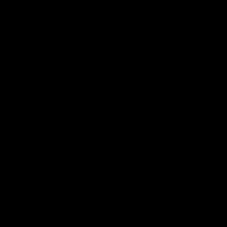
\includegraphics[scale=0.25]{square.jpg}
\caption{The pairwise nature of the Born radius.}
\label{sq}
\end{figure}%

See \cref{sq}.

Lorem ipsum dolor sit amet, consectetur adipiscing elit, sed do eiusmod tempor incididunt ut labore et dolore magna aliqua. Feugiat vivamus at augue eget arcu. Donec et odio pellentesque diam volutpat commodo sed egestas egestas. Sem nulla pharetra diam sit amet. Sagittis purus sit amet volutpat consequat mauris. 

\begin{info} % Information block
	This is an interesting piece of information, to which the reader should pay special attention. Fusce varius orci ac magna dapibus porttitor. In tempor leo a neque bibendum sollicitudin. Nulla pretium fermentum nisi, eget sodales magna facilisis eu. Praesent aliquet nulla ut bibendum lacinia. Donec vel mauris vulputate, commodo ligula ut, egestas orci. Suspendisse commodo odio sed hendrerit lobortis. Donec finibus eros erat, vel ornare enim mattis et.
\end{info}

\begin{table}[ht]
	\centering
	\caption{Gravimetric analysis of silver halides in a 1.27-mL sample of Salton Sea water.}
		\begin{tabular}{rSSScS}
			\toprule
				\multicolumn{1}{c}{}             & \multicolumn{4}{c}{Test Tubes}\\
				\cmidrule(rl){2-5} 
					Qty of Sample                & A             & B             & C             & D      & Avg             \\
				\cmidrule(r){1-1} \cmidrule(rl){2-5} \cmidrule(l){6-6}
					Mass (g)                     & 1.399         & 1.32          & 1.328         & 1.408  & 1.364           \\
					Density (g/mL)               & 1.10          & 1.04          & 1.05          & 1.109  & 1.07            \\
					Mass w/ Precipitate (g)      & 13.443        & 13.401        & 13.348        & ---    & 13.397          \\
					Mass AgCl (\num{e-2} g)      & 9.0           & 9.2           & 8.7           & ---    & 8.9             \\
					Moles AgCl (\num{e-4} mol)   & 6.28          & 6.42          & 6.08          & ---    & 6.50            \\
			\bottomrule
		\end{tabular}
	\label{tabgrav}
\end{table}
 
% tikz figure - https://www.mathcha.io/editor#
\begin{figure}[htbp]
	\centering
		% code generated by https://www.mathcha.io/editor#


% Gradient Info
  
\tikzset {_fl3j1z7ci/.code = {\pgfsetadditionalshadetransform{ \pgftransformshift{\pgfpoint{0 bp } { 0 bp }  }  \pgftransformscale{1 }  }}}
\pgfdeclareradialshading{_ajvec99hy}{\pgfpoint{0bp}{0bp}}{rgb(0bp)=(0,0,0);
rgb(0.17857142857142858bp)=(0,0,0);
rgb(25bp)=(1,1,1);
rgb(400bp)=(1,1,1)}
\tikzset{_c47t8m2b3/.code = {\pgfsetadditionalshadetransform{\pgftransformshift{\pgfpoint{0 bp } { 0 bp }  }  \pgftransformscale{1 } }}}
\pgfdeclareradialshading{_kz6fsyt8x} { \pgfpoint{0bp} {0bp}} {color(0bp)=(transparent!27);
color(0.17857142857142858bp)=(transparent!27);
color(25bp)=(transparent!0);
color(400bp)=(transparent!0)} 
\pgfdeclarefading{_sdra5fwgv}{\tikz \fill[shading=_kz6fsyt8x,_c47t8m2b3] (0,0) rectangle (50bp,50bp); } 
\tikzset{every picture/.style={line width=0.65pt}} %set default line width to 0.75pt        

\begin{tikzpicture}[x=0.75pt,y=0.75pt,yscale=-1,xscale=1]
%uncomment if require: \path (0,300); %set diagram left start at 0, and has height of 300

%Shape: Circle [id:dp5031363586176847] 
\draw  [fill={rgb, 255:red, 0; green, 0; blue, 0 }  ,fill opacity=1 ] (353.67,159.68) .. controls (353.67,157.75) and (355.23,156.18) .. (357.17,156.18) .. controls (359.1,156.18) and (360.67,157.75) .. (360.67,159.68) .. controls (360.67,161.61) and (359.1,163.18) .. (357.17,163.18) .. controls (355.23,163.18) and (353.67,161.61) .. (353.67,159.68) -- cycle ;
%Shape: Circle [id:dp6021592429793765] 
\draw  [fill={rgb, 255:red, 225; green, 225; blue, 225 }  ,fill opacity=1 ] (345,159.33) .. controls (345,157.4) and (346.57,155.83) .. (348.5,155.83) .. controls (350.43,155.83) and (352,157.4) .. (352,159.33) .. controls (352,161.27) and (350.43,162.83) .. (348.5,162.83) .. controls (346.57,162.83) and (345,161.27) .. (345,159.33) -- cycle ;
%Shape: Circle [id:dp03262422408388033] 
\path  [shading=_ajvec99hy,_fl3j1z7ci,path fading= _sdra5fwgv ,fading transform={xshift=2}] (200,203.5) .. controls (200,176.53) and (221.86,154.67) .. (248.83,154.67) .. controls (275.8,154.67) and (297.67,176.53) .. (297.67,203.5) .. controls (297.67,230.47) and (275.8,252.33) .. (248.83,252.33) .. controls (221.86,252.33) and (200,230.47) .. (200,203.5) -- cycle ; % for fading 
 \draw  [color={rgb, 255:red, 255; green, 255; blue, 255 }  ,draw opacity=1 ] (200,203.5) .. controls (200,176.53) and (221.86,154.67) .. (248.83,154.67) .. controls (275.8,154.67) and (297.67,176.53) .. (297.67,203.5) .. controls (297.67,230.47) and (275.8,252.33) .. (248.83,252.33) .. controls (221.86,252.33) and (200,230.47) .. (200,203.5) -- cycle ; % for border 

%Shape: Circle [id:dp6125886336785793] 
\draw  [fill={rgb, 255:red, 0; green, 0; blue, 0 }  ,fill opacity=1 ] (247.37,202.04) .. controls (247.37,201.23) and (248.02,200.57) .. (248.83,200.57) .. controls (249.64,200.57) and (250.3,201.23) .. (250.3,202.04) .. controls (250.3,202.84) and (249.64,203.5) .. (248.83,203.5) .. controls (248.02,203.5) and (247.37,202.84) .. (247.37,202.04) -- cycle ;
%Shape: Rectangle [id:dp737374784788116] 
\draw   (320,150) -- (390,150) -- (390,182.36) -- (320,182.36) -- cycle ;
%Straight Lines [id:da9404773687410686] 
\draw [fill={rgb, 255:red, 255; green, 255; blue, 255 }  ,fill opacity=1 ]   (320,150) -- (320,182.36) -- (248.83,202.04) ;
%Shape: Polygon [id:ds005534302931645474] 
\draw  [fill={rgb, 255:red, 255; green, 255; blue, 255 }  ,fill opacity=1 ] (320,182.36) -- (390,182.36) -- (248.83,202.04) -- cycle ;
%Shape: Circle [id:dp39755043985132055] 
\draw  [fill={rgb, 255:red, 0; green, 0; blue, 0 }  ,fill opacity=1 ] (344,163.83) .. controls (344,161.9) and (345.57,160.33) .. (347.5,160.33) .. controls (349.43,160.33) and (351,161.9) .. (351,163.83) .. controls (351,165.77) and (349.43,167.33) .. (347.5,167.33) .. controls (345.57,167.33) and (344,165.77) .. (344,163.83) -- cycle ;
%Shape: Circle [id:dp4473204849748251] 
\draw  [fill={rgb, 255:red, 225; green, 225; blue, 225 }  ,fill opacity=1 ] (348,166.51) .. controls (348,164.58) and (349.57,163.01) .. (351.5,163.01) .. controls (353.43,163.01) and (355,164.58) .. (355,166.51) .. controls (355,168.45) and (353.43,170.01) .. (351.5,170.01) .. controls (349.57,170.01) and (348,168.45) .. (348,166.51) -- cycle ;
%Shape: Circle [id:dp4488461328919484] 
\draw  [fill={rgb, 255:red, 0; green, 0; blue, 0 }  ,fill opacity=1 ] (349,161.5) .. controls (349,159.57) and (350.57,158) .. (352.5,158) .. controls (354.43,158) and (356,159.57) .. (356,161.5) .. controls (356,163.43) and (354.43,165) .. (352.5,165) .. controls (350.57,165) and (349,163.43) .. (349,161.5) -- cycle ;
%Shape: Circle [id:dp7389549254976258] 
\draw  [fill={rgb, 255:red, 225; green, 225; blue, 225 }  ,fill opacity=1 ] (353.67,163.18) .. controls (353.67,161.25) and (355.23,159.68) .. (357.17,159.68) .. controls (359.1,159.68) and (360.67,161.25) .. (360.67,163.18) .. controls (360.67,165.11) and (359.1,166.68) .. (357.17,166.68) .. controls (355.23,166.68) and (353.67,165.11) .. (353.67,163.18) -- cycle ;
%Shape: Circle [id:dp479134066231107] 
\draw  [fill={rgb, 255:red, 0; green, 0; blue, 0 }  ,fill opacity=1 ] (344.5,170.01) .. controls (344.5,168.08) and (346.07,166.51) .. (348,166.51) .. controls (349.93,166.51) and (351.5,168.08) .. (351.5,170.01) .. controls (351.5,171.95) and (349.93,173.51) .. (348,173.51) .. controls (346.07,173.51) and (344.5,171.95) .. (344.5,170.01) -- cycle ;
%Shape: Circle [id:dp4479985418514103] 
\draw  [fill={rgb, 255:red, 225; green, 225; blue, 225 }  ,fill opacity=1 ] (340.5,167.33) .. controls (340.5,165.4) and (342.07,163.83) .. (344,163.83) .. controls (345.93,163.83) and (347.5,165.4) .. (347.5,167.33) .. controls (347.5,169.27) and (345.93,170.83) .. (344,170.83) .. controls (342.07,170.83) and (340.5,169.27) .. (340.5,167.33) -- cycle ;
%Shape: Circle [id:dp7971297276833167] 
\draw  [fill={rgb, 255:red, 0; green, 0; blue, 0 }  ,fill opacity=1 ] (353.67,166.68) .. controls (353.67,164.75) and (355.23,163.18) .. (357.17,163.18) .. controls (359.1,163.18) and (360.67,164.75) .. (360.67,166.68) .. controls (360.67,168.61) and (359.1,170.18) .. (357.17,170.18) .. controls (355.23,170.18) and (353.67,168.61) .. (353.67,166.68) -- cycle ;
%Shape: Circle [id:dp5729729111609032] 
\draw  [fill={rgb, 255:red, 225; green, 225; blue, 225 }  ,fill opacity=1 ] (349.5,172) .. controls (349.5,170.07) and (351.07,168.5) .. (353,168.5) .. controls (354.93,168.5) and (356.5,170.07) .. (356.5,172) .. controls (356.5,173.93) and (354.93,175.5) .. (353,175.5) .. controls (351.07,175.5) and (349.5,173.93) .. (349.5,172) -- cycle ;
%Shape: Circle [id:dp07629231382977153] 
\draw  [fill={rgb, 255:red, 0; green, 0; blue, 0 }  ,fill opacity=1 ] (353,172) .. controls (353,170.07) and (354.57,168.5) .. (356.5,168.5) .. controls (358.43,168.5) and (360,170.07) .. (360,172) .. controls (360,173.93) and (358.43,175.5) .. (356.5,175.5) .. controls (354.57,175.5) and (353,173.93) .. (353,172) -- cycle ;
%Shape: Circle [id:dp14599951094051478] 
\draw  [fill={rgb, 255:red, 225; green, 225; blue, 225 }  ,fill opacity=1 ] (357.17,170.18) .. controls (357.17,168.25) and (358.73,166.68) .. (360.67,166.68) .. controls (362.6,166.68) and (364.17,168.25) .. (364.17,170.18) .. controls (364.17,172.11) and (362.6,173.68) .. (360.67,173.68) .. controls (358.73,173.68) and (357.17,172.11) .. (357.17,170.18) -- cycle ;
%Straight Lines [id:da98323072818843] 
\draw    (248.83,202.04) -- (320,150) ;




\end{tikzpicture}
 
		\caption{The nucleus.}
		\label{fig:bornrad}
\end{figure}

Tellus in hac habitasse platea. Lectus quam id leo in vitae turpis massa sed. A condimentum vitae sapien pellentesque habitant morbi tristique. Velit sed ullamcorper morbi tincidunt. Volutpat est velit egestas dui id ornare arcu. Ipsum dolor sit amet consectetur adipiscing elit duis tristique. Tellus orci ac auctor augue mauris augue neque. 

Vestibulum morbi blandit cursus risus at. Ornare lectus sit amet est placerat. Quam viverra orci sagittis eu volutpat odio facilisis mauris. Posuere ac ut consequat semper viverra nam libero justo laoreet. Phasellus egestas tellus rutrum tellus pellentesque eu tincidunt. Interdum varius sit amet mattis. Massa sapien faucibus et molestie ac feugiat sed lectus. Tellus cras adipiscing enim eu. Non diam phasellus vestibulum lorem.

% ==========================================================================================
% ==========================================================================================
% ==========================================================================================

\subsection{Procedure}

Eget aliquet nibh praesent tristique magna sit amet purus gravida. Sed viverra tellus in hac. Aliquet porttitor lacus luctus accumsan tortor posuere ac ut. Neque laoreet suspendisse interdum consectetur libero id. Amet risus nullam eget felis eget nunc lobortis mattis. Etiam sit amet nisl purus. Sit amet consectetur adipiscing elit ut aliquam purus. Eu lobortis elementum nibh tellus molestie nunc non. Egestas tellus rutrum tellus pellentesque eu tincidunt tortor aliquam nulla. Vitae suscipit tellus mauris a diam. Ut pharetra sit amet aliquam id diam maecenas ultricies mi. Suspendisse faucibus interdum posuere lorem.

% ==========================================================================================
% ==========================================================================================
% ==========================================================================================

\subsection{Materials}

Amet mauris commodo quis imperdiet. Facilisi nullam vehicula ipsum a arcu cursus. Sit amet dictum sit amet justo donec enim. Ac turpis egestas integer eget aliquet nibh. A arcu cursus vitae congue mauris. Augue lacus viverra vitae congue eu consequat ac. Congue quisque egestas diam in arcu cursus euismod quis. Tempus quam pellentesque nec nam. Pellentesque habitant morbi tristique senectus et netus et malesuada fames. Venenatis tellus in metus vulputate eu. Maecenas sed enim ut sem viverra aliquet eget. Quam lacus suspendisse faucibus interdum posuere lorem. Gravida dictum fusce ut placerat orci nulla. Tristique sollicitudin nibh sit amet commodo nulla facilisi nullam vehicula. Pretium lectus quam id leo in vitae turpis massa.

%notice the syntax

\begin{equation}
\label{eq:born}
\underbrace{text-above}_{text-below}
\end{equation}

\begin{equation}
\label{eq:bornp}
\underset{text-below}{text-above}
\end{equation}

\begin{equation*}
\underbrace{\ce{CH3Cl}}_{\textnormal{electrophile}} + \underbrace{\ce{NaOH}}_{\textnormal{nucleophile}} \hskip-.5em\ce{-> CH3OH + NaCl}
\end{equation*}


\begin{center}
\ce{
Zn^2+
<=>[+ 2OH-][+ 2H+]
$\underset{\text{amphoteres Hydroxid}}{\ce{Zn(OH)2 v}}$
->[+ 2OH-][+ 2H+]
$\underset{\text{Hydroxozikat}}{\ce{[Zn(OH)4]^2-}}$
+ H2 ^
}
\end{center} 


% ==========================================================================================
% ==========================================================================================
% ==========================================================================================

\begin{comment} % natbib/manual
\newpage
\addcontentsline{toc}{section}{References}
\bibliographystyle{plain}
\begin{thebibliography}{200}
\mytref{heitlon}{Heitler, W.; London, F.}{Wechselwirkung neutraler Atome und hom\"oopolare Bindung nach der Quantenmechanik}{Phys.\ Lett.}{1927}{44}{455--473}
\myzref{ez}{Terhorst, J.\ P.; Jorgensen, W.\ L.}{\textsl{E/Z} Energetics for Molecular Modeling and Design}{J.\ Chem.\ Theory Comput.}{2010}{6}{9}{2762--2769}
\end{thebibliography}
\end{comment}

% biber/biblatex
\printbibliography

% ==========================================================================================
% ==========================================================================================
% ==========================================================================================

\end{document}















% ==========================================================================================
% ==========================================================================================
% ==========================================================================================


% ==========================================================================================
% ==========================================================================================
% ==========================================================================================

% notes

%          with symbol, use \footnote[2]{text}
%          instead of 2 you can put the number of the symbol you like:
%          1   asterisk *   
%          2   dagger  
%          3   double dagger  
%          4   section symbol §   
%          5   paragraph ¶   
%          6   parallel lines  
%          7   two asterisks 
%          8   two daggers 
%          9   two double daggers 

% some fancy chem notation examples

\begin{center}
\ce{
Zn^2+
<=>[+ 2OH-][+ 2H+]
$\underset{\text{amphoteres Hydroxid}}{\ce{Zn(OH)2 v}}$
<=>[+ 2OH-][+ 2H+]
$\underset{\text{Hydroxozikat}}{\ce{[Zn(OH)4]^2-}}$
+ H2 ^
}
\end{center}    

% align environment

\begin{align*}
\ce{ A + B &->[+e] C \\
C &->[+e] D + E }
\end{align*}

